\documentclass{article}
\usepackage{amsmath}
\usepackage{amssymb}
\usepackage{graphicx}
\usepackage{hyperref}
\usepackage[version=4]{mhchem}

\title{Example 4}
\date{}

\begin{document}
\maketitle

(AMC) In the figure, \(A B C D\) is an isosceles trapezoid with side lengths \(A D=B C=5, A B=4\), and \(D C=10\). The point \(C\) is on \(D F\) and \(B\) is the midpoint of hypotenuse \(\overline{D E}\) in the right triangle \(D E F\). Then \(C F=\)\\
(A) 3.25\\
(B) 3.5\\
(C) 3.75\\
(D) 4.0\\
(E) 4.25\\
\centering
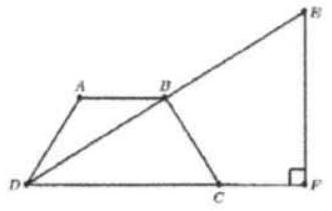
\includegraphics[width=\textwidth]{images/076(1).jpg}

Solution: (D).\\
Method 1:\\
Drop perpendiculars \(\overline{A G}\) and \(\overline{B H}\) to \(\overline{D F}\). Then \(G H=4\), so \(D G=H C=\frac{1}{2}(D C-G H)=3\)\\
(b)\\
(A) \(7+\frac{2}{3} \sqrt{3}\)\\
(B) 8\\
(C) \(9 \frac{1}{2}\)\\
(E) \(8+3 \sqrt{3}\)\\
(B) 8\\
(C) \(9 \frac{1}{2}\)\\
(D) \(8+\sqrt{3}\)\\
(D) \(8+\sqrt{3}\)

\[
-\ln
\]

都\\
\centering
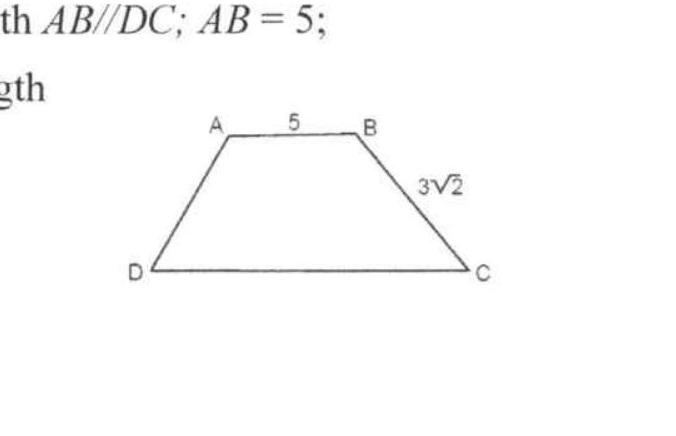
\includegraphics[width=\textwidth]{images/076.jpg}


Since \(\overline{B H} / / \overline{E F}\) and \(B\) is in midpoint of \(D E\), it follows that \(H\) is the midpoint of \(D F\). Thus, \(D H=D G+G H=3+4\) and \(D F=2 D H=14\), so \(C F=D F-D C=14-10=4\).

Method 2:\\
Drop perpendiculars \(A G\) and \(B H\) to \(D F\) and connect \(B F\).\\
Then \(G H=4\), so \(D G=H C=\frac{1}{2}(D C-G H)=3\). Since \(B D\) \(=B F\), triangle \(D B F\) is isosceles, and so \(D H=H F\) and \(C F=\)\\
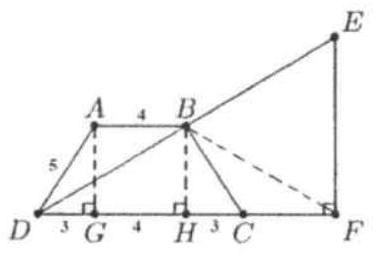
\includegraphics[width=\textwidth]{images/077(2).jpg} 4.


\end{document}
